% !TEX program = pdflatex
% Build:  pdflatex report.tex   (run twice for the table of contents)
%   or:   tectonic report.tex   (single pass, fetches packages on demand)

\documentclass[11pt,a4paper]{article}

\usepackage[utf8]{inputenc}
\usepackage[T1]{fontenc}
\usepackage{lmodern}
\usepackage[english]{babel}
\usepackage[margin=2.5cm]{geometry}
\usepackage{microtype}
\usepackage{xcolor}
\usepackage{graphicx}
\usepackage{listings}
\usepackage{booktabs}
\usepackage{array}
\usepackage{tabularx}
\usepackage{enumitem}
\usepackage{tikz}
\usetikzlibrary{positioning, arrows.meta, shapes.geometric, fit, backgrounds}
\usepackage{fancyhdr}
\usepackage[hidelinks]{hyperref}

% --- Listings styling -------------------------------------------------------
\definecolor{codebg}{RGB}{246,247,249}
\definecolor{codekw}{RGB}{32, 80, 160}
\definecolor{codecm}{RGB}{105, 115, 125}
\definecolor{codestr}{RGB}{160, 60, 60}

\lstdefinelanguage{batch}{
  morekeywords={set,setlocal,enabledelayedexpansion,if,not,exist,for,do,
                echo,mkdir,del,rmdir,call,goto,pause,exit,errorlevel,
                in,equ,gtr,lss},
  morecomment=[l]{::},
  morecomment=[l]{REM},
  morestring=[b]",
  sensitive=false,
}

\lstset{
  basicstyle=\ttfamily\footnotesize,
  backgroundcolor=\color{codebg},
  keywordstyle=\color{codekw}\bfseries,
  commentstyle=\color{codecm}\itshape,
  stringstyle=\color{codestr},
  frame=single,
  rulecolor=\color{codebg!75!black},
  framesep=4pt,
  breaklines=true,
  breakatwhitespace=true,
  columns=fullflexible,
  showstringspaces=false,
  xleftmargin=4pt,
  xrightmargin=4pt,
  aboveskip=8pt,
  belowskip=8pt,
}

% --- Page style -------------------------------------------------------------
\pagestyle{fancy}
\fancyhf{}
\fancyhead[L]{transcodeVR}
\fancyhead[R]{Project Report}
\fancyfoot[C]{\thepage}
\renewcommand{\headrulewidth}{0.4pt}

% --- Title metadata ---------------------------------------------------------
\title{
  \vspace{-1.5cm}
  \textbf{transcodeVR} \\[0.3em]
  \large A Batch Pipeline for VR-to-Flat Video Conversion \\
  \large via FFmpeg
}
\author{michel-ch}
\date{2026}

% ===========================================================================
\begin{document}

\maketitle
\thispagestyle{empty}

\vspace{0.5cm}
\begin{abstract}
\noindent
\textbf{transcodeVR} is a small set of Windows batch scripts that drive
\texttt{FFmpeg} to reproject 180\textdegree{} side-by-side stereoscopic
video into a flat 2D rectilinear ``normal-camera'' view, with optional
per-folder concatenation of the resulting clips. A third script provides
a hardware-accelerated 1080p downscale for ordinary footage. The project
intentionally has no build system, no runtime dependencies beyond
\texttt{FFmpeg}, and no source code in the conventional sense: every entry
point is a self-contained \texttt{.bat} file. This report describes the
goal of the project, the architecture of the solution, the
\texttt{FFmpeg} pipeline used to perform the reprojection, and the
trade-offs that shaped the design.
\end{abstract}

\tableofcontents
\newpage

% ===========================================================================
\section{Goal}

The project addresses a personal-archival problem: turning recordings
made on a 180\textdegree{} stereoscopic VR camera into ordinary,
playable, shareable 2D video files. VR sources stored as
\emph{half-equirectangular} side-by-side (SBS) frames look distorted
and unwatchable in conventional players, and even on VR-aware players
they require a headset to be enjoyed.

\subsection{Stated objectives}
\begin{enumerate}[leftmargin=1.5em, itemsep=0.2em]
  \item \textbf{Reproject} 180\textdegree{} SBS source video to a flat
        rectilinear view, with framing tuned for an arbitrary
        camera mount (\textit{e.g.} a head-mounted rig looking at a
        subject below the eyeline).
  \item \textbf{Batch} the conversion across nested folders, so an
        entire archive of source clips can be processed unattended.
  \item \textbf{Optionally concatenate} the per-clip outputs of each
        scene folder into a single playable file, since many VR
        recordings are split into multiple sequential takes.
  \item \textbf{Strip identifying metadata} from outputs so files do not
        carry over camera/serial/handler information.
  \item Provide a \textbf{secondary downscale path} for non-VR footage
        that needs to be reduced to 1080p.
\end{enumerate}

\subsection{Non-goals}
\begin{itemize}[leftmargin=1.5em, itemsep=0.2em]
  \item No GUI. The user interface is the \texttt{.bat} file.
  \item No cross-platform support. Windows-only.
  \item No content management. The scripts treat folders as opaque
        units; they do not parse filenames, dates, or sidecar metadata.
  \item No incremental processing. Re-running a script re-encodes
        everything; checkpointing was deliberately skipped to keep the
        scripts trivial.
\end{itemize}

% ===========================================================================
\section{Architecture}

\subsection{High-level view}

The solution is composed of three independent batch-file entry points,
each a thin orchestrator around a single \texttt{FFmpeg} invocation
template. The two VR scripts share an input/output convention
(\texttt{vr/} $\rightarrow$ \texttt{nonevr/}) and an encoder template;
the 1080p script is conventionally separate (\texttt{input/}
$\rightarrow$ \texttt{output/}, NVENC instead of x264).

\begin{figure}[h]
\centering
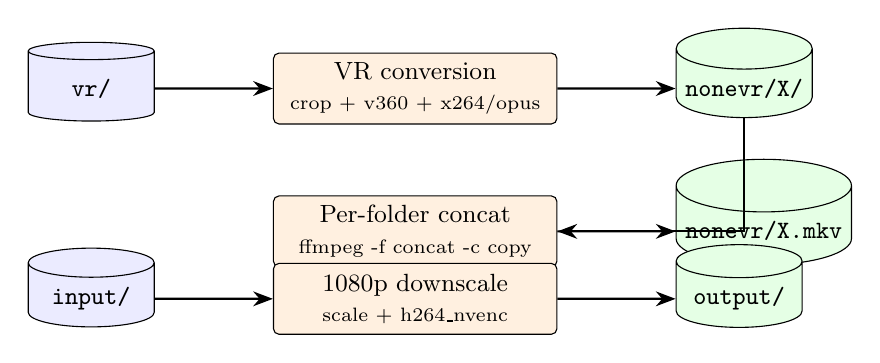
\begin{tikzpicture}[
  node distance=0.9cm and 1.5cm,
  every node/.style={font=\small},
  io/.style={cylinder, shape border rotate=90, draw, minimum width=1.6cm,
             minimum height=1.0cm, fill=blue!8, aspect=0.3},
  proc/.style={rectangle, draw, rounded corners=2pt, minimum width=3.6cm,
               minimum height=0.9cm, fill=orange!12, align=center},
  outc/.style={cylinder, shape border rotate=90, draw, minimum width=1.6cm,
               minimum height=1.0cm, fill=green!10, aspect=0.3},
  arrow/.style={-{Stealth[length=2.5mm]}, thick},
]

  \node[io]   (vr)        {\texttt{vr/}};
  \node[proc, right=of vr] (vrconv) {VR conversion \\ \scriptsize crop $+$ v360 $+$ x264/opus};
  \node[outc, right=of vrconv] (nonevrf) {\texttt{nonevr/X/}};
  \node[proc, below=of vrconv] (merge) {Per-folder concat \\ \scriptsize ffmpeg -f concat -c copy};
  \node[outc, right=of merge] (nonevrm) {\texttt{nonevr/X.mkv}};

  \node[io,   below=1.6cm of vr] (input) {\texttt{input/}};
  \node[proc, right=of input] (down) {1080p downscale \\ \scriptsize scale $+$ h264\_nvenc};
  \node[outc, right=of down] (output) {\texttt{output/}};

  \draw[arrow] (vr) -- (vrconv);
  \draw[arrow] (vrconv) -- (nonevrf);
  \draw[arrow] (nonevrf.south) |- (merge.east);
  \draw[arrow] (merge) -- (nonevrm);
  \draw[arrow] (input) -- (down);
  \draw[arrow] (down) -- (output);

\end{tikzpicture}
\caption{High-level dataflow. Both VR scripts share the \texttt{vr/}
$\rightarrow$ \texttt{nonevr/} path; only \texttt{VR2Normal.bat}
includes the optional per-folder concat stage. The 1080p script is
fully independent.}
\label{fig:dataflow}
\end{figure}

\subsection{Components}

\begin{table}[h]
\centering
\renewcommand{\arraystretch}{1.25}
\begin{tabularx}{\linewidth}{lXl}
\toprule
\textbf{Script} & \textbf{Responsibility} & \textbf{Output} \\
\midrule
\texttt{VR2Normal.bat} & Convert every VR clip in every subfolder of
\texttt{vr/}, then concatenate the resulting clips per-folder into a
single MKV. & \texttt{nonevr/X/*.mkv}, \texttt{nonevr/X.mkv} \\
\texttt{only\_vr.bat} & Same per-clip conversion as
\texttt{VR2Normal.bat}, without the concat stage. Used when each clip
must remain a separate output. & \texttt{nonevr/X/*.mkv} \\
\texttt{only\_1080p.bat} & Hardware-accelerated 1080p downscale of
\texttt{*.MP4} files in \texttt{input/}. Audio stream-copied. &
\texttt{output/X/*\_1080p.MP4} \\
\bottomrule
\end{tabularx}
\caption{The three entry-point scripts and their roles.}
\end{table}

The two VR scripts share the per-clip encoder line verbatim; the only
difference between them is whether the concat stage runs after every
folder is processed. This duplication is deliberate: keeping each
script self-contained means the user can run either one without
worrying about an extra flag, and editing the encoder parameters in
both files is a two-edit operation.

\subsection{Folder convention}

\begin{lstlisting}[language=batch, caption={Project layout. Empty
content directories ship with the repository as conventions; only
\texttt{*.bat}, \texttt{LICENSE}, \texttt{README.md}, and the
\texttt{docs/} tree are tracked in git.}]
transcodeVR/
   VR2Normal.bat       :: VR convert + per-folder concat
   only_vr.bat         :: VR convert (no concat)
   only_1080p.bat      :: 1080p downscale (NVENC)
   vr/                 :: VR input  (one subfolder per scene)
   nonevr/             :: VR output
   input/              :: 1080p input
   output/             :: 1080p output
   temp/               :: concat lists (auto-deleted)
   docs/               :: markdown docs
   report/             :: this report
\end{lstlisting}

The "one level of subfolders" model is the unifying convention: the
input root is always a directory of \emph{scene folders}, never of
loose files. This lets the script use a simple two-level
\texttt{for /d} loop and assigns clear semantics to a folder
(``everything inside is one scene'').

% ===========================================================================
\section{The FFmpeg pipeline}

\subsection{Per-clip VR conversion}

The heart of the project is a single \texttt{FFmpeg} command applied to
every input clip. It is broken across two filter stages followed by a
re-encode.

\begin{lstlisting}[caption={Per-clip VR conversion command (line-broken
for readability; in the source it is one line).}]
ffmpeg
  -hide_banner -loglevel error -stats
  -y
  -hwaccel cuda
  -i <input>
  -map 0:v:0 -map 0:a
  -vf "crop=w=iw/2:h=ih:x=0:y=0,
       v360=hequirect:flat:in_stereo=2d:out_stereo=2d:
            iv_fov=180:ih_fov=180:d_fov=115:
            pitch=-35:yaw=0:roll=0:
            w=2560:h=1440:interp=lanczos:reset_rot=1"
  -c:v libx264 -preset medium -crf 24 -tune film
  -x264-params keyint=600:bframes=7
  -c:a libopus -b:a 128K
  -map_metadata:g -1
  -map_metadata:s:v -1
  -map_metadata:s:a 0:s:a
  -metadata:s "HANDLER_NAME="
  <output>.mkv
\end{lstlisting}

\subsubsection{Stage 1: crop the right eye away}

\noindent
180\textdegree{} SBS sources place the left eye in the left half of the
frame and the right eye in the right half. Since the project produces
\emph{monoscopic} output, only one eye is needed. The
\texttt{crop=iw/2:ih:0:0} step keeps the left half. Switching to the
right eye is a single edit (\texttt{x=0} $\rightarrow$ \texttt{x=iw/2}).

\subsubsection{Stage 2: reproject hemisphere to plane}

\noindent
The cropped image is then a \emph{half-equirectangular} projection of
the camera's viewing hemisphere. \texttt{FFmpeg}'s \texttt{v360} filter
converts it to a rectilinear view (the \texttt{flat} target):

\vspace{0.4em}
\begin{center}
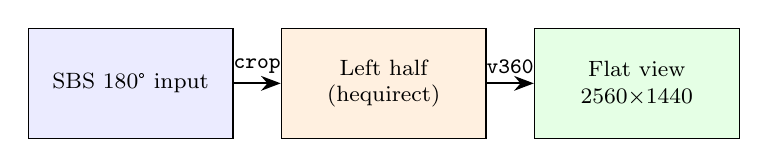
\begin{tikzpicture}[
  every node/.style={font=\footnotesize, align=center},
  arrow/.style={-{Stealth[length=2.5mm]}, thick}
]
  \node (sbs) [draw, fill=blue!8, minimum width=2.6cm,
               minimum height=1.4cm] {SBS 180\textdegree{} input};
  \node[right=0.6cm of sbs] (crop) [draw, fill=orange!12,
       minimum width=2.6cm, minimum height=1.4cm] {Left half \\ (hequirect)};
  \node[right=0.6cm of crop] (flat) [draw, fill=green!10,
       minimum width=2.6cm, minimum height=1.4cm] {Flat view \\ 2560$\times$1440};
  \draw[arrow] (sbs) -- node[above]{\texttt{crop}} (crop);
  \draw[arrow] (crop) -- node[above]{\texttt{v360}} (flat);
\end{tikzpicture}
\end{center}
\vspace{0.4em}

\noindent
The framing parameters control where the virtual camera looks inside
the source hemisphere:

\begin{table}[h]
\centering
\renewcommand{\arraystretch}{1.25}
\begin{tabular}{llp{8cm}}
\toprule
\textbf{Param} & \textbf{Value} & \textbf{Effect} \\
\midrule
\texttt{iv\_fov,ih\_fov} & 180,180 & Source covers the full hemisphere
(both axes). \\
\texttt{d\_fov} & 115 & Output diagonal field of view; smaller is
``zoomed in,'' larger is ``wide angle.'' \\
\texttt{pitch} & $-35$ & Tilt down 35\textdegree{}, compensating for a
camera mounted at eye level looking at a subject below. \\
\texttt{yaw,roll} & 0,0 & No pan, no roll. \\
\texttt{w,h} & 2560,1440 & 1440p output. \\
\texttt{interp} & \texttt{lanczos} & High-quality resampling. \\
\texttt{reset\_rot} & 1 & Discard any source-side rotation metadata. \\
\bottomrule
\end{tabular}
\caption{The \texttt{v360} parameters and their visual effect.}
\end{table}

These four numbers (\texttt{d\_fov}, \texttt{pitch}, \texttt{yaw},
\texttt{roll}) are the only ``creative'' inputs to the pipeline; all
other settings are quality/encoding choices.

\subsubsection{Stage 3: encode}

\noindent
Video is encoded with software x264:
\textbf{preset medium}, \textbf{CRF 24}, \textbf{tune film},
\textbf{keyint 600}, \textbf{7 B-frames}. Audio is re-encoded with
\textbf{libopus} at \textbf{128 kbps}. The output container is
\textbf{Matroska} (\texttt{.mkv}) because it tolerates Opus and
arbitrary stream layouts cleanly, and because the merge step uses
\texttt{ffmpeg -f concat -c copy}, which is most reliable on MKV.

A subtle but useful detail is the metadata stripping at the end:
\texttt{-map\_metadata:g~-1}, \texttt{-map\_metadata:s:v~-1}, and
\texttt{-metadata:s~"HANDLER\_NAME="} together remove globally-scoped
container metadata, all per-stream video metadata, and the
\texttt{HANDLER\_NAME} tag that some cameras populate with
serial-number-like strings. This makes outputs more anonymous and less
likely to confuse downstream players.

\subsection{Concatenation stage}

\noindent
After per-clip conversion, \texttt{VR2Normal.bat} walks each output
folder, builds a concat list with \texttt{dir /b /on} (alphabetical),
and runs:

\begin{lstlisting}
ffmpeg -hide_banner -loglevel error -stats
       -f concat -safe 0
       -i <concat_list.txt>
       -c copy
       <merged>.mkv
\end{lstlisting}

\noindent
Critically, this does \emph{not} re-encode. Because every per-clip
output was produced by the same \texttt{FFmpeg} command, all clips
share identical codec parameters, and \texttt{-c copy} can stitch them
without re-encoding. This makes the merge essentially a memcpy of
demuxed packets, and runs at I/O speed. Folders containing zero or one
file skip the concat step.

The alphabetical ordering is intentionally simple: it relies on the
naming discipline of the source clips. Zero-padded numeric names
(\texttt{clip01.mp4}, \texttt{clip02.mp4}, \dots) sort correctly,
while bare numeric names (\texttt{clip1.mp4}, \texttt{clip10.mp4},
\texttt{clip2.mp4}) do not.

\subsection{1080p downscale pipeline}

\noindent
The 1080p script is intentionally a different shape:

\begin{lstlisting}
ffmpeg -y -i <input>
       -vf "scale=1920:1080"
       -c:v h264_nvenc -preset p4 -cq 23
       -c:a copy
       <output>_1080p.MP4
\end{lstlisting}

\noindent
Two notable design choices: encoding is \textbf{NVENC} (GPU)
rather than x264, trading a small amount of bit-efficiency for a large
speedup; and audio is \textbf{stream-copied}, since downscaling does
not require touching audio. The output extension is preserved as
\texttt{.MP4} (since audio is unmodified, no container change is
needed).

% ===========================================================================
\section{Trade-offs}

The project deliberately optimizes for \textbf{hackability over
robustness}. Some of the consequences:

\begin{itemize}[leftmargin=1.5em, itemsep=0.4em]
  \item \textbf{No idempotency}: re-running a script reprocesses every
        file, even if an output already exists. A \texttt{if exist
        skip} would be one line, but was deliberately omitted to keep
        the user's mental model trivial: \emph{nuke the output folder
        if you want to start over.}
  \item \textbf{No exit code}: each script ends in \texttt{pause}, with
        no propagation of \texttt{errorlevel} to the caller. The scripts
        are intended for interactive use, not pipeline automation.
  \item \textbf{Hardcoded paths}: \texttt{FFMPEG\_PATH} is baked into
        the VR scripts, and all input/output roots are absolute paths
        rooted at \texttt{C:\textbackslash Users\textbackslash
        \%USERNAME\%\textbackslash Desktop\textbackslash transcodeVR}.
        Moving the project requires editing the scripts.
  \item \textbf{Mixed FFmpeg invocation}: the VR scripts use a
        configurable \texttt{FFMPEG\_PATH}; the 1080p script calls
        \texttt{ffmpeg} from \texttt{PATH}. This is technical debt
        rather than a design choice.
  \item \textbf{Inconsistent folder conventions} across the VR and
        1080p scripts (\texttt{vr/}/\texttt{nonevr/} vs.
        \texttt{input/}/\texttt{output/}). Each pipeline is internally
        consistent, but they cannot share a folder.
  \item \textbf{Silent quirks} (\textit{e.g.} the unused
        \texttt{!THREADS!} variable in \texttt{only\_1080p.bat},
        the misleading ``\_MERGED.mkv'' string in
        \texttt{VR2Normal.bat}'s success message) are documented in
        \texttt{docs/troubleshooting.md} rather than fixed, on the
        principle that the scripts are working code in production
        use and edits must be ``surgical.''
\end{itemize}

% ===========================================================================
\section{Conclusion}

\noindent
\texttt{transcodeVR} is, in the end, a deliberately small project: ~250
lines of batch script plus an \texttt{FFmpeg} filter chain. The
architectural decisions in this report (one-level folder convention,
duplicated encoder template across two scripts, no idempotency, no
exit codes) are all chosen to keep the system trivial to read and edit.
The complexity that does exist lives almost entirely in the
\texttt{FFmpeg} command line: the \texttt{v360} reprojection, the
metadata-stripping flags, the concat-list construction. Everything
else is a thin loop around it.

The full markdown documentation lives at \texttt{docs/} in the project
root and is the authoritative source for usage; this report is a
high-level companion that describes \emph{why} the system has the
shape it does.

\vspace{1cm}
\noindent\textbf{Project repository:}\ \url{https://github.com/michel-ch/transcodeVR}

\end{document}
